Le but du jeu est d'avoir plus de points que l'adversaire au bout de 5/20/30 tours (selon la difficulté). Chaque joueur commence avec un certain nombre d'unités (également selon la difficulté) qu'il pourra déplacer à chaque tour afin d'occuper plus de cases ou de détruire des unités adverses. Le placement de chaque unité rapporte plus ou moins de points.

\subsection{Carte du monde}

Les unités se déplaceront sur une carte de taille variable selon la difficulté. Les cases seront hexagonales [\textsc{figure~\ref{cases}}], les unités auront donc au maximum 6 déplacements/attaques possibles. IL existe trois types de tuile possible : plaine, forêt et montagne. Les différentes races auront des interactions spéciales avec ces tuiles.

\begin{figure}[!h]
\centering
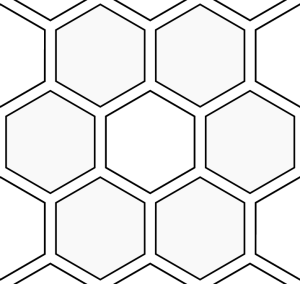
\includegraphics[width=0.5\textwidth]{img/hexagonal.png}
\caption{Cases de la carte}
\label{cases}
\end{figure}

\subsection{Lancement du jeu}

Au lancement du jeu, le joueur peut soit : \newline créer une nouvelle partie, soit en charger une comme l'explique le \textsc{diagramme~\ref{lancement}}. Lors de la création d'une nouvelle partie, le joueur peut personnaliser sa partie de différentes façons, lui permettant d'avoir des expériences différentes à chaque partie. Il peut tout d'abord choisir la difficulté, ce qui influence plusieurs paramètres :

\begin{itemize}
  \item Démo    :   6x6 cases ;  5 tours ; 4 unités par peuple
  \item Petite  : 10x10 cases ; 20 tours ; 6 unités par peuple
  \item Normale : 14x14 cases ; 30 tours ; 8 unités par peuple
\end{itemize}

\clearpage
Chaque joueur peut ensuite choisir sa race parmi les 3 races disponibles : Elfe, orc et nain. Chaque race confère des bonus détaillés en partie 2 de ce rapport.

\begin{figure}[!h]
\centering
\label{lancement}
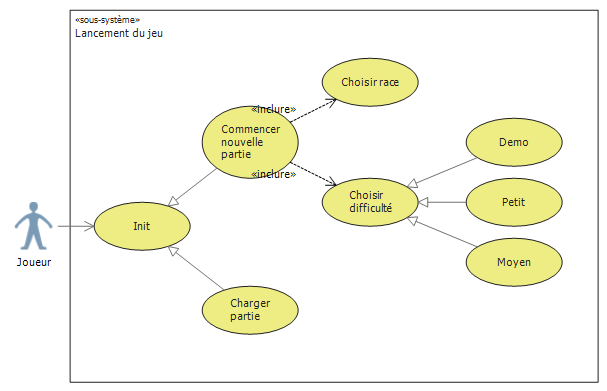
\includegraphics[width=1\textwidth]{img/LancementDuJeu.png}
\caption{Lancement du jeu}
\end{figure}

\subsection{Déroulement d'un tour}

Nous allons maintenant expliciter le déroulement d'un tour. A chaque tour, le joueur peut déplacer chaque unité qu'il contrôle si celle-ci a des points de déplacement. Si une unité adverse est sur une case adjacente, il peut à la place attaquer cette unité pour tenter de prendre le contrôle de cette case. Le déroulement des combats est expliqué dans la partie suivante de ce rapport.


